\documentclass{article}

\usepackage[utf8]{inputenc}
\usepackage[russian]{babel}
\usepackage{graphicx}
\usepackage{subcaption}
\usepackage{amsmath}

\newcommand{\geff}{\gamma_{eff}}
\newcommand{\Ps}{\mathcal P}

\begin{document}
\title{Пространственная зависимость спин-тюна}
\maketitle

Из COSY Infinity мы имеем функцию спин-тюна $\nu_s(\vec z)$ в виде разложения ряда Тэйлора, где
\begin{align*}
  \vec z &= (x,a,y,b,\ell,\delta), \\
  \ell &= -(t - t_0)v_0\frac{\gamma-1}{\gamma}, \\
  \delta &= \frac{\Delta K}{K}.
\end{align*}

Мы проверяем следующую гипотезу \#0: функцию спин-тюна $\nu_s(\vec z)$ многих переменных можно свести к
функции одной сложной переменной $\nu_s(\geff)$.

Преположим, что мы не знаем формальное выражение параметра $\geff$; но в любом случае, если гипотеза \#0 верна,
то существует система координат (одной из осей которых является $\nu_s$), в которой частицы,
совершающие бетатронные колебания в горизонтальной плоскости неотличимы с точки зрения спин-тюна от частиц,
совершающих колебания в вертикальной плоскости.

К тому же, в этой системе координат не должны присутствовать координаты из поперечного
фазового пространства $(x,y)$, и $(y,b)$.

Таким образом, будем рассматривать пространство $\Ps=(\ell, \delta, \nu_s)$. Если гипотеза \#0 верна,
траектории частиц в поперечном фазовом пространстве не должны отражаться на траектории частиц в $\Ps$.

\section{Результаты симуляции}
Здесь представлены результаты анализа данных теста по проверке спин-тюн эквивалентности частиц
с разными траекториями но одинаковыми равновесными уровнями энергии. Сетап симуляции описан в
разделе 2.5 диссертации.

На Рисунке~\ref{fig:main:all_ps} изображена зависимость $\nu_s(\vec z)$ от $(\ell, \delta)$ в том случае, когда
$\vec z$ представляет реальную фазовую координату частицы в ускорителе. Мы наблюдаем:
\begin{enumerate}
\item стратификацию среднего уровня спин-тюна, как мы это видели в симуляциях по подавлению декогеренции
  в разделе 2.2.6;
  \item стратификация гораздо значительнее для X-банча (синий), чем для Y-банча (красный).
\end{enumerate}

Последнее объясняется большим значением функции дисперсии в горизонтальной плоскости.

\begin{figure}[h]
  \centering
  \begin{subfigure}{\linewidth}\centering
    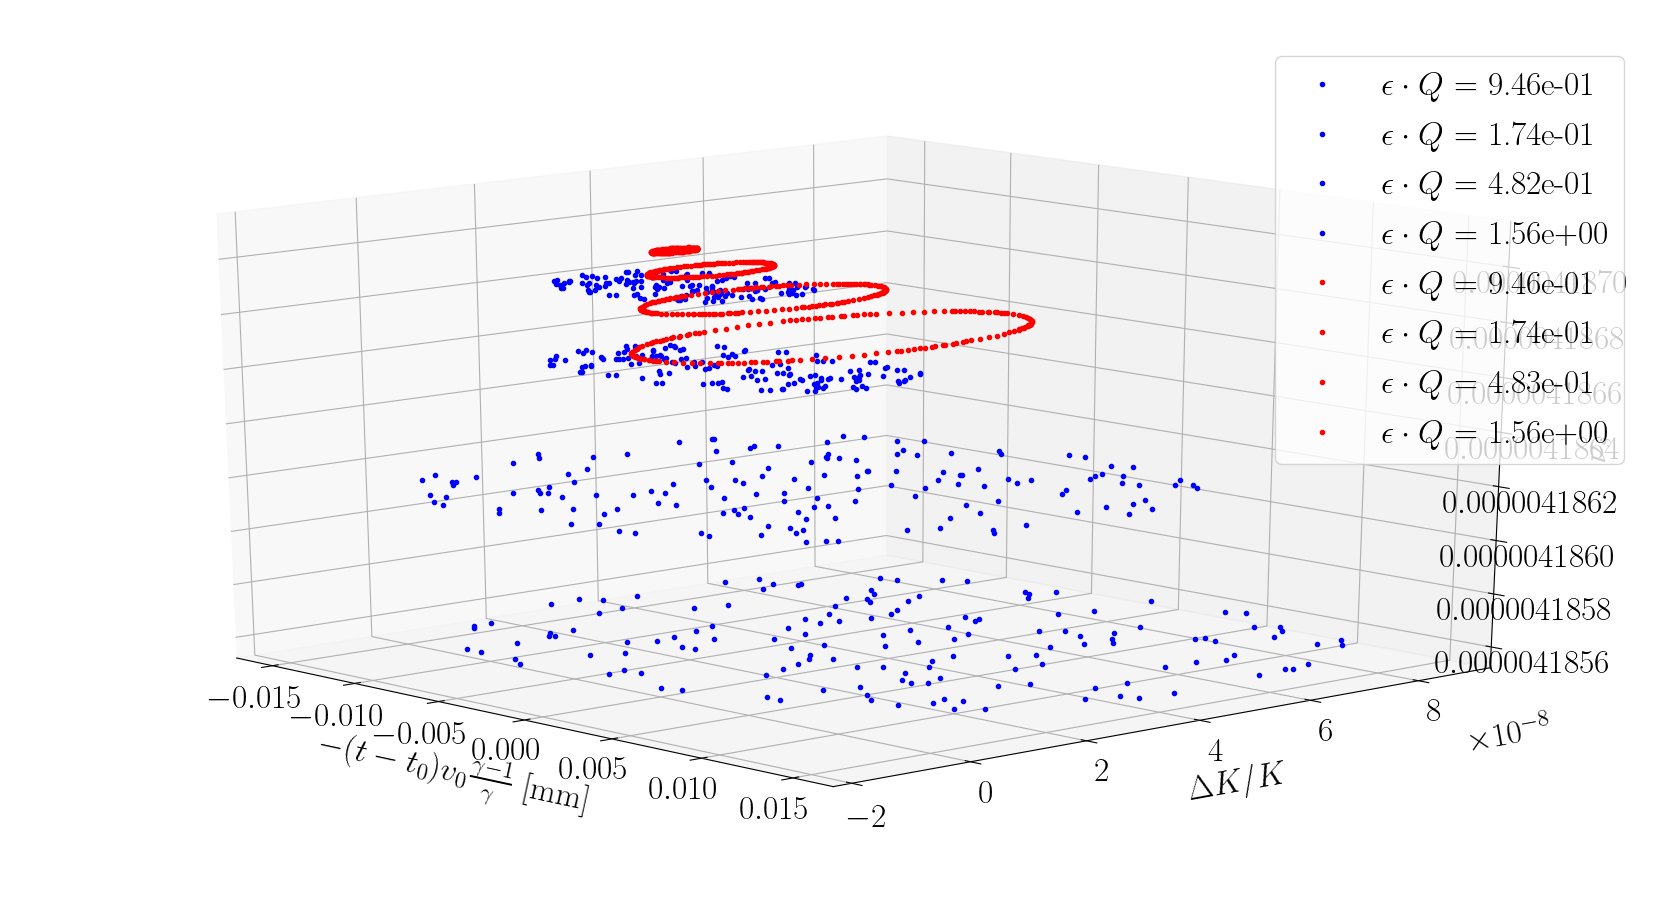
\includegraphics[height=.3\paperheight]{../../img/STUNE_TRAJ_TEST/3D_plot_all_ps_vars}
    \caption{Использованы все переменные фазового пространства.\label{fig:main:all_ps}}
  \end{subfigure}
  \begin{subfigure}{\linewidth}\centering
    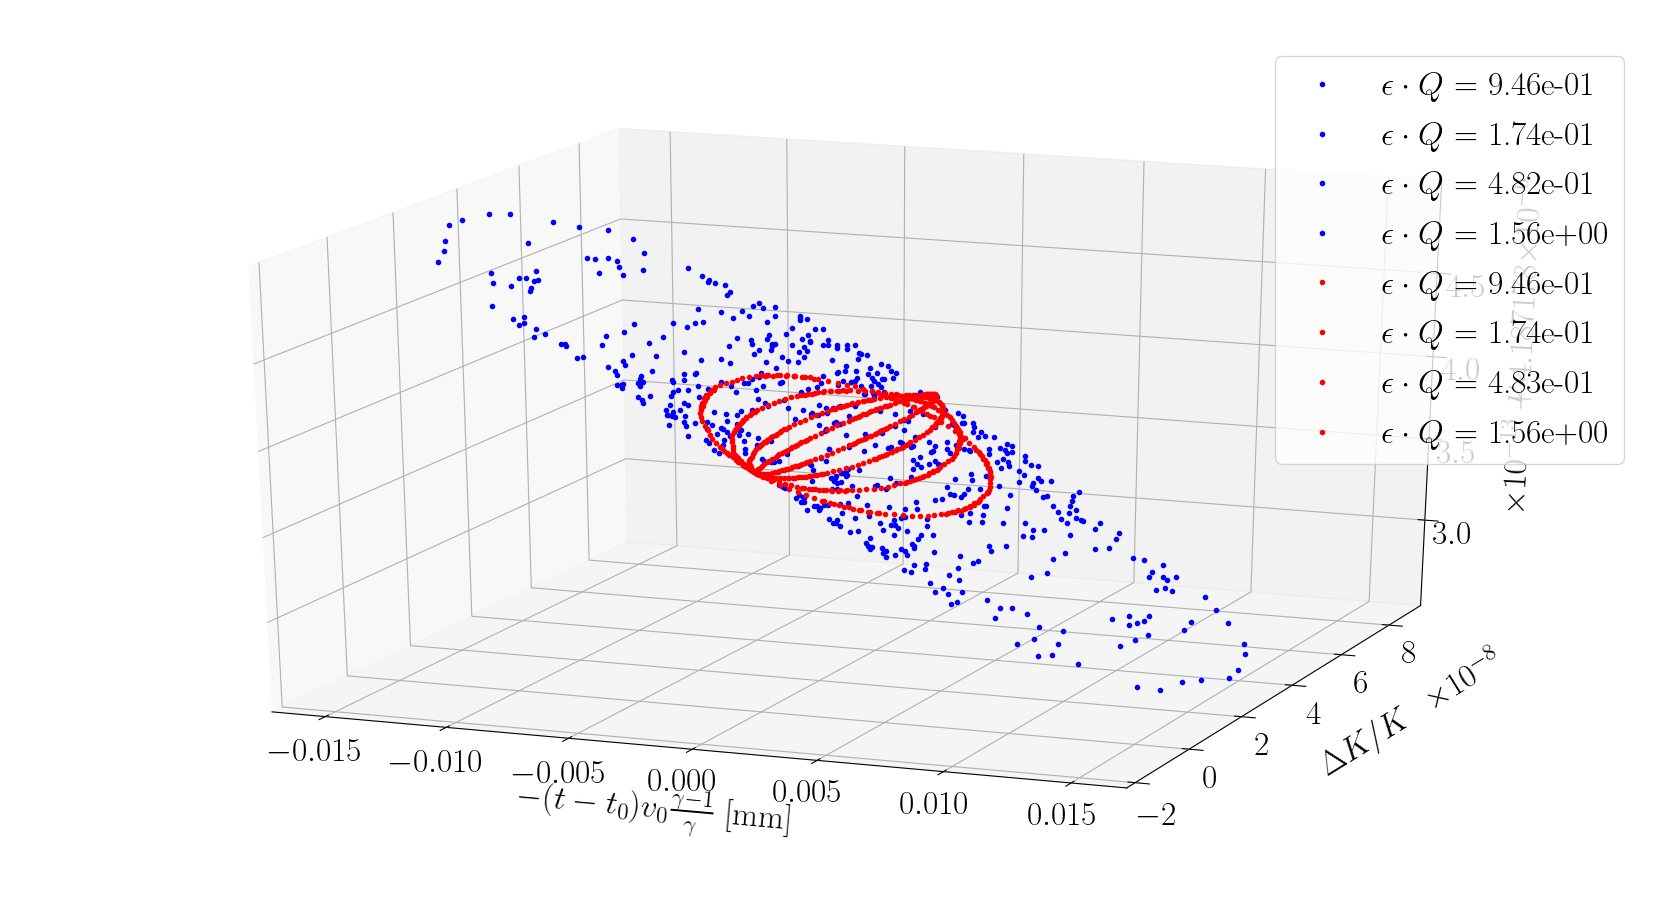
\includegraphics[height=.3\paperheight]{../../img/STUNE_TRAJ_TEST/3D_plot_only_long_ps_vars}
    \caption{Использованы только переменные продольного фазового пространства.\label{fig:main:long_ps}}
  \end{subfigure}
  \caption{Зависимость спин-тюна частицы от её положения в продольном фазовом пространстве.\label{fig:main}}
\end{figure}

На Рисунке~\ref{fig:main:long_ps} изображена та же зависимость, но только в этот раз
$\vec z = (0, 0, 0, 0, \ell, \delta)$, т.е. функция взята только на проекции фазовых эллипсов частиц на плоскость
продольного фазового пространства. Таким образом, функция спин-тюна не различает поперечные фазовые пространства
пучков. Мы видим, что в этом случае спин-тюны обоих пучков лежат в одной и той же плоскости.

Отметим, что при построении рисунков использовались частицы с одинаковым произведением поперечного эмиттанса на
бетатронный тюн (значения указаны на легенде), т.е. приблизительно равного удлинения орбиты,
если расчитывать его по формуле
\[
\left(\frac{\Delta L}{L}\right)_\beta = \frac{\pi}{2L}[\epsilon_x\cdot Q_x + \epsilon_y\cdot Q_y].
\]

(\emph{Приблизительно}, потому что частицы Y-банча имеют малый (на уровне $\le10^{-10}$ м$\cdot$рад), но ненулевой
эмиттанс в $(x,a)$, которым я пренебрегаю.)

Данные рисунки получены из структуры с выключенными сексеуполями, однако такая же картина (нестратифицированный
спин-тюн в наклонённой плоскости) наблюдается в случае использования оптимизированного семейства соответствующих
секступолей в структуре.

\begin{figure}[h]
  \centering
  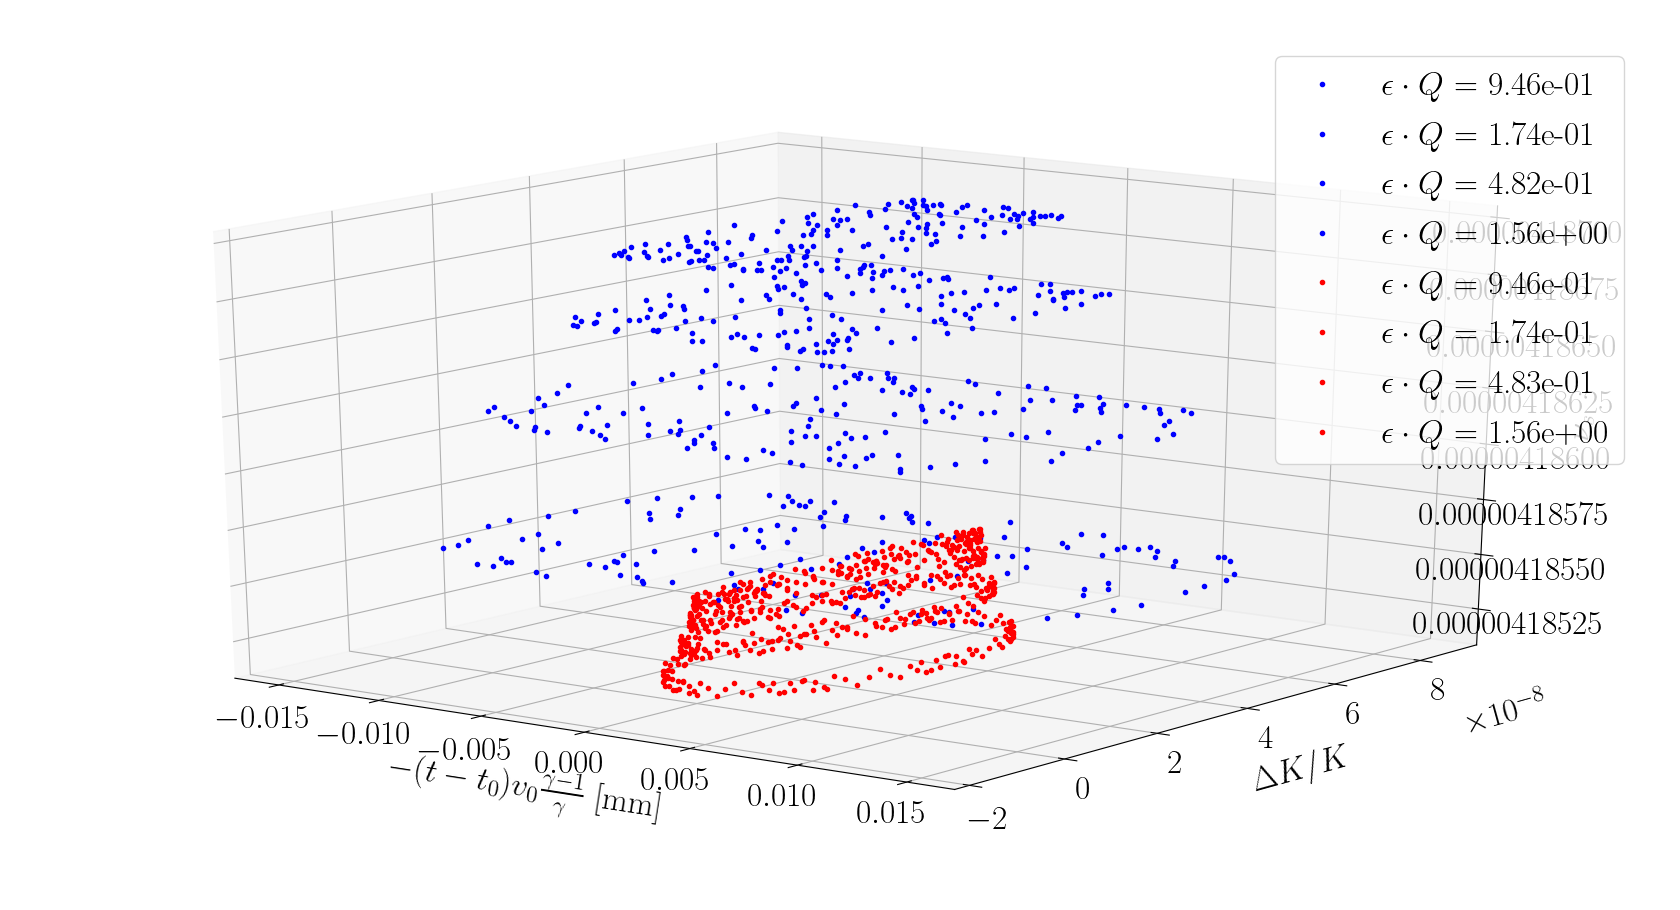
\includegraphics[height=.3\paperheight]{../../img/STUNE_TRAJ_TEST/3D_plot_long_+_trans_ps(for_bunch)}
  \caption{Использованы переменные продольного и соответствующего банчу поперечного (для Y-банча (Y, B),
    для X-банча (X, A)) фазового пространства.\label{fig:secondary}}
\end{figure}

На Рисунке~\ref{fig:secondary} изображена та же самая зависимость, но в этот раз, при вычислении спин-тюнов
к координатам продольного фазового пространства добавлялись координаты соответствующего пучку поперечного
фазового пространства, т.е. для Y-банча, $\vec z = (0, 0, y, b, \ell, \delta)$,
для X-банча $\vec z = (x, a, 0, 0, \ell, \delta)$. Снова появляется стратификация.

\begin{figure}[h]
  \centering
  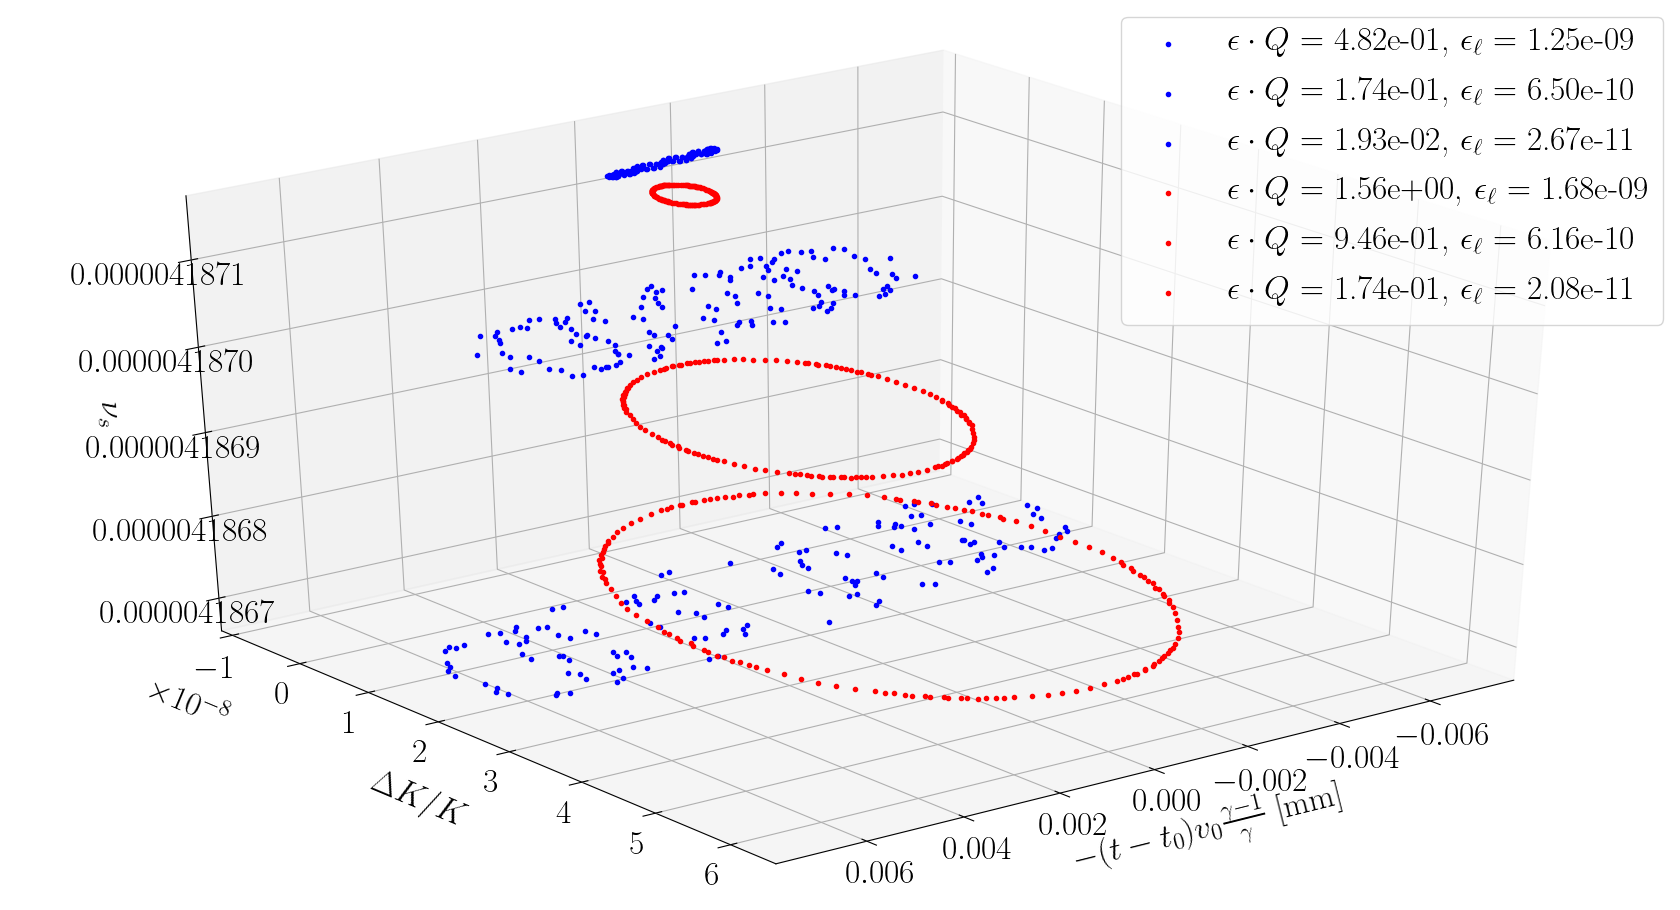
\includegraphics[height=.3\paperheight]{../../img/STUNE_TRAJ_TEST/3D_plot_all_ps_vars_equal_long_emi}
  \caption{Подобраны траектории с приблизительно равными продольными эмиттансами.\label{fig:gamma_eff}}
\end{figure}

\section{Вывод}
Мы наблюдаем на Рисунке~\ref{fig:gamma_eff}, что частицы, с приблизительно одинаковыми продольныим эмиттансами
имеют приблизительно одинаковый уровень спин-тюна, независимо от плоскости совершения бетатронных колебаний.

Таким образом, гипотеза \#0 подтверждена.

\end{document}
